% A triangulation (left) and a sub-division with a hanging vertex (right).
% Shared by the lecture notes and the slides.
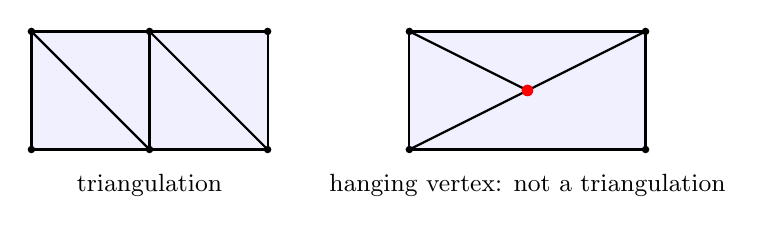
\begin{tikzpicture}[scale=1.5]
    \fill[blue!6] (0,0) rectangle (2,1);
    \draw[thick] (0,0) -- (2,0) -- (2,1) -- (0,1) -- cycle;
    \draw[thick] (1,0) -- (1,1);
    \draw[thick] (0,1) -- (1,0) (1,1) -- (2,0);
    \foreach \p in {(0,0),(1,0),(2,0),(0,1),(1,1),(2,1)} \fill \p circle (.9pt);
    \node at (1,-.3) {\small triangulation};
    \begin{scope}[xshift=3.2cm]
        \fill[blue!6] (0,0) rectangle (2,1);
        \draw[thick] (0,0) -- (2,0) -- (2,1) -- (0,1) -- cycle;
        \draw[thick] (0,0) -- (2,1);
        \draw[thick] (0,1) -- (1,.5);
        \foreach \p in {(0,0),(2,0),(0,1),(2,1)} \fill \p circle (.9pt);
        \fill[red] (1,.5) circle (1.4pt);
        \node at (1,-.3) {\small hanging vertex: not a triangulation};
    \end{scope}
\end{tikzpicture}
